\documentclass[aspectratio=169]{beamer}
\usepackage[T1]{fontenc}
\usepackage[utf8]{inputenc}
\usepackage{listings}
\usepackage{colortbl}

\definecolor{codegreen}{rgb}{0,0.6,0}
\definecolor{codegray}{rgb}{0.5,0.5,0.5}
\definecolor{codepurple}{rgb}{0.58,0,0.82}
\definecolor{backcolour}{rgb}{0.95,0.95,0.92}

\lstdefinestyle{mystyle}{
    backgroundcolor=\color{backcolour},
    commentstyle=\color{codegreen},
    keywordstyle=\color{magenta},
    numberstyle=\tiny\color{codegray},
    stringstyle=\color{codepurple},
    basicstyle=\ttfamily\footnotesize,
    breakatwhitespace=false,
    breaklines=false,
    captionpos=b,
    keepspaces=true,
    numbers=left,
    numbersep=5pt,
    showspaces=false,
    showstringspaces=false,
    showtabs=false,
    tabsize=2
}

\lstdefinestyle{yaml}{
    basicstyle=\color{blue}\footnotesize,
    string=[s]{'}{'},
    comment=[l]{:},
    morecomment=[l]{\-},
    backgroundcolor=\color{backcolour},
    commentstyle=\color{codegreen},
    keywordstyle=\color{magenta},
    numberstyle=\tiny\color{codegray},
    stringstyle=\color{codepurple},
    basicstyle=\ttfamily\footnotesize,
    breakatwhitespace=false,
    breaklines=false,
    captionpos=b,
    keepspaces=true,
    numbers=left,
    numbersep=5pt,
    showspaces=false,
    showstringspaces=false,
    showtabs=false,
    tabsize=2
 }

\lstdefinestyle{ww}{
    basicstyle=\color{blue}\footnotesize,
    morestring=[b]{"},
    comment=[s]{.}{\ },
    morecomment=[s]{.}{\}},
    morecomment=[s]{\$}{\ },
    morecomment=[s]{\$}{\}},
    backgroundcolor=\color{backcolour},
    commentstyle=\color{codegreen},
    keywordstyle=\color{magenta},
    numberstyle=\tiny\color{codegray},
    stringstyle=\color{codegreen},
    basicstyle=\ttfamily\footnotesize,
    breakatwhitespace=false,
    breaklines=false,
    captionpos=t,
    keepspaces=true,
    numbers=left,
    numbersep=5pt,
    showspaces=false,
    showstringspaces=false,
    showtabs=false,
    tabsize=2,
    keywords={if,range,end},
 }

\lstdefinestyle{wwctl}{
    language=bash,
    basicstyle=\color{blue}\footnotesize,
    backgroundcolor=\color{backcolour},
    commentstyle=\color{codegreen},
    keywordstyle=\color{magenta},
    numberstyle=\tiny\color{codegray},
    stringstyle=\color{codegreen},
    basicstyle=\ttfamily\footnotesize,
    breakatwhitespace=false,
    breaklines=true,
    captionpos=t,
    keepspaces=true,
    numbers=left,
    numbersep=5pt,
    showspaces=false,
    showstringspaces=false,
    showtabs=false,
    tabsize=2,
    morestring=[s]{\ W}{=},
    keywords={wwctl,container,import,shell,export,node,add,set,list},
 }



\lstset{style=mystyle}

\title{Warewulf\\
making cluster\\
installations fast and \\
reliable}
\date{April 25, Ostrava}
\author{Christian Goll <\texttt{cgoll@suse.com}>}
\usetheme{suse}

\begin{document}

\begin{frame}
\titlepage
\end{frame}
\begin{frame}[fragile]
\frametitle{Introduction}
\framesubtitle{Warewulf is tool for managing Beowulf clusters}
\begin{columns}
\column{0.7\textwidth}
\begin{block}{Beowulf}
  \begin{itemize}
    \item old british poem
  \end{itemize}
\end{block}
\begin{block}{Beowulf cluster}
  \begin{itemize}
    \item became popular in the 90.
    \item use of the shelf hardware
    \begin{itemize}
      \item 486 \& Linux \textbf{not} Cray \& Unix
    \end{itemize}
    \item Warewulf is a typo of werewolf
    \item Caos Linux \& Warewulf were designed for Beowulf clusters
    \item Caos Linux evolved into CentOS
    \begin{itemize}
      \item Gregory Kurtzner started developement of Warewulf v4
    \end{itemize}
  \end{itemize}
\end{block}
\column{0.3\textwidth}
  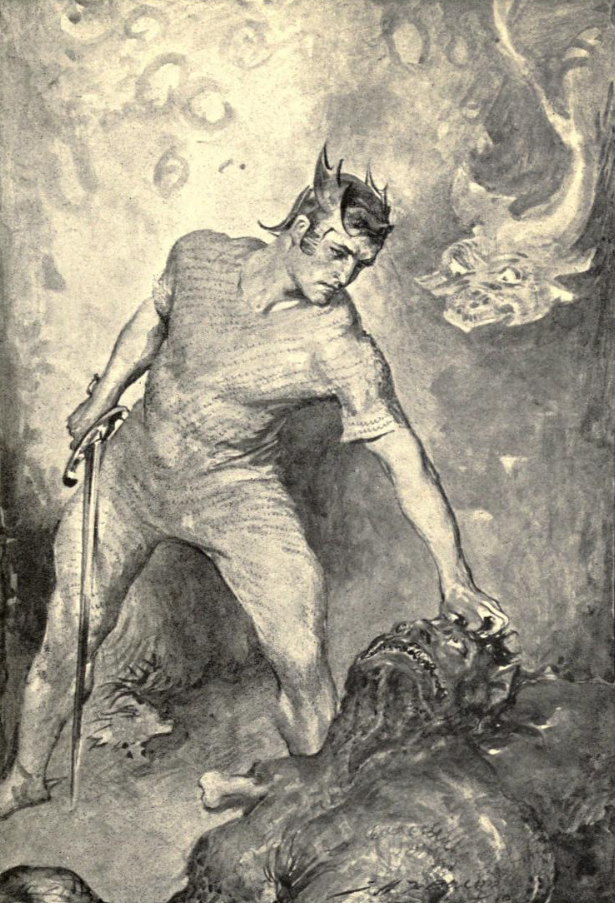
\includegraphics[width=\linewidth]{Beowulf}
\end{columns}
\end{frame}

\begin{frame}[fragile]
\frametitle{Introduction}
\framesubtitle{HPC landscape}
\begin{block}{Top five Supercomputers}
\begin{table}
\begin{tabular}{c|l|l|l|l}
1 &	Frontier& EPYC 64C &AMD MI250X &Slingshot-11 \\
2 &	Aurora  & Xeon 9470 & Intel GPU Max&Slingshot-11 \\
3 &	Eagle & Xeon 8480 &  NVIDIA H100 & NVIDIA Infiniband \\
\rowcolor{backcolour}
4 &	Fugaku &  A64FX 48C 2.2GHz & - & Tofu interconnect D \\
5 &	LUMI &  EPYC 64C 2GHz & AMD MI250X & Slingshot-11 
\end{tabular}
\end{table}
\begin{itemize}
  \item only Fugaku uses non standard CPU
  \item others are Beowulf clusters with GPUs attached
\end{itemize}
\end{block}
\end{frame}
\begin{frame}[fragile]
\frametitle{Introduction}
\framesubtitle{Beowulf cluster}
\begin{columns}
\column{0.5\textwidth}
\begin{block}{Base components}
\begin{itemize}
  \item management node
  \item compute nodes
  \item management network
  \item network boot (PXE)
\end{itemize}
\end{block}
\begin{block}{Optional components}
\begin{itemize}
  \item more compute nodes
  \item fast network interconnects 
  \item central storage
  \item bmc/ipmi
\end{itemize}
\end{block}
\column{0.5\textwidth}
  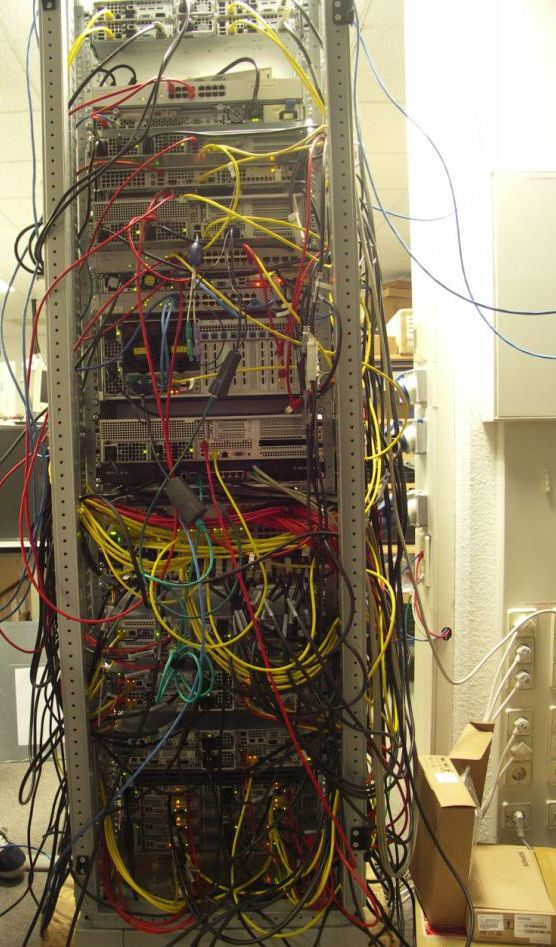
\includegraphics[width=.6\linewidth]{Transtec-056}
\end{columns}
\end{frame}
\begin{frame}[fragile]
\frametitle{Introduction}
\framesubtitle{Beowulf Cluster}
\begin{columns}
\column{0.5\textwidth}
\begin{block}{Differences to data centers}
  \begin{itemize}
    \item compute nodes are cattle
    \begin{itemize}
      \item parallel/MPI require identical nodes
    \end{itemize}
    \item hierarchical organization
    \item compute are not updated after boot process
    \item applications come from central storage
    \item applications are self compiled with tools like \texttt{spack} \& \texttt{EasyBuild}
  \end{itemize}
\end{block}
\column{0.5\textwidth}
  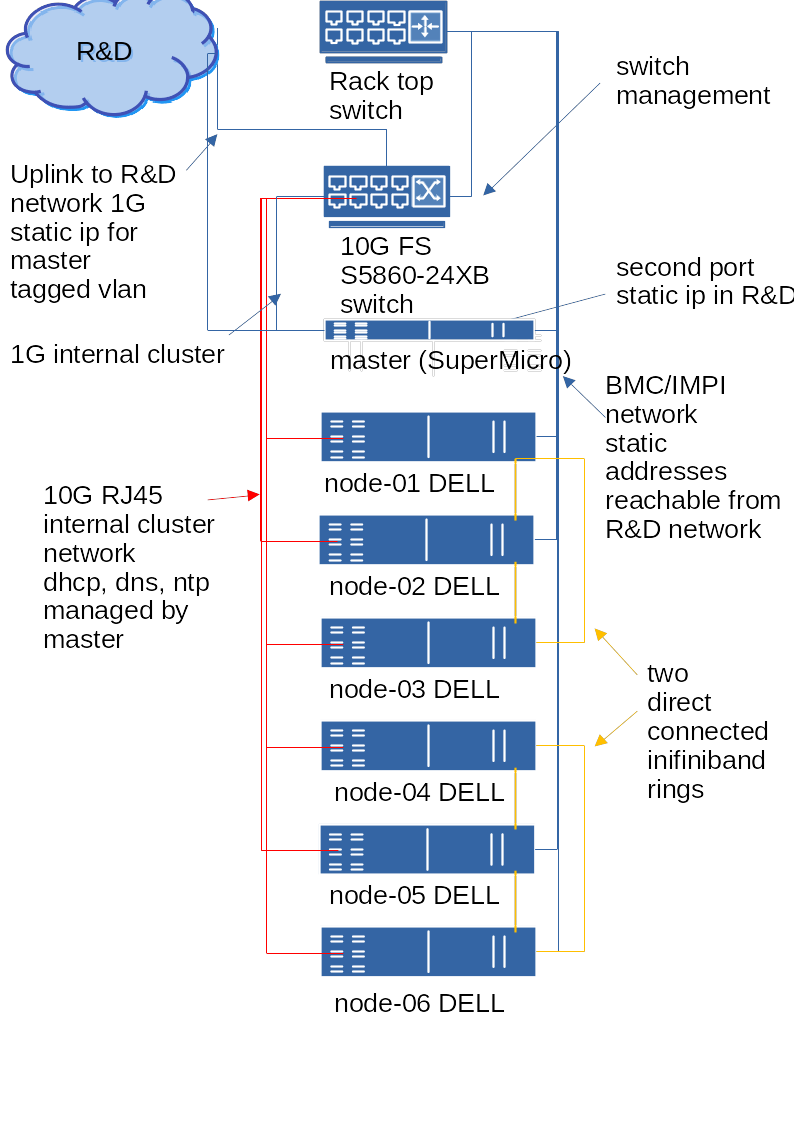
\includegraphics[width=.6\linewidth]{networkplan}
\end{columns}
\end{frame}
\begin{frame}[fragile]
\frametitle{Warewulf description}
\framesubtitle{Software stack}
\begin{columns}
\column{0.6\textwidth}
  \begin{block}{Warewulf components}
  \hspace*{.1\linewidth}\begin{minipage}{.8\linewidth}
  \begin{block}{Compute nodes}
    \textbf{boot from network into tmpfs}
  \end{block}
  \begin{block}{Warewulfd delivers}
    \begin{itemize}
      \item kernel \& modules
      \item node image
      \item node configurations
    \end{itemize}
  \end{block}
  \begin{block}{\texttt{wwctl} cmd line tool}
    \begin{itemize}
      \item manages node database
      \item manages node image
    \end{itemize}
  \end{block}
  \end{minipage}
  \end{block}
\column{0.4\textwidth}
  \begin{block}{external components}
  \hspace*{.1\linewidth}\begin{minipage}{.8\linewidth}
    \begin{block}{Dhcp server}
      \begin{itemize}
      \item ISC \texttt{dhcpd} server
      \item \texttt{dnsmasq}
    \end{itemize}
    \end{block}
    \begin{block}{tftp}
      \begin{itemize}
      \item tftp from \texttt{kernel.org}
      \item dnsmasq
    \end{itemize}
    \end{block}
  \end{minipage} 
  \end{block}
  \begin{block}{Optional}
    \begin{itemize}
      \item nfs
      \item manage \texttt{/etc/hosts}
    \end{itemize}
  \end{block}
\end{columns}
\end{frame}

\begin{frame}[fragile]
\frametitle{Warewulf configuration}
\framesubtitle{database \texttt{/etc/warewulf/nodes.conf}}
\begin{columns}
\column{0.5\textwidth}
\begin{itemize}
  \item plain yaml file
  \item easy backup
  \item can be version controlled
  \item external tools support
  \begin{itemize}
    \item vim, ansible
  \end{itemize}
\end{itemize}
\begin{block}{Profiles}
\begin{itemize}
  \item stores identical values for collection of nodes
  \item values can be overridden on node basis
\end{itemize}
\end{block}
\column{0.5\textwidth}
\begin{lstlisting}[style=yaml]
WW_INTERNAL: 45
nodeprofiles:
  default:
    comment: This profile is automatically included for each node
    container name: leap
    network devices:
      default:
        device: eth0
nodes:
  n01:
    profiles:
    - default
    network devices:
      default:
        hwaddr: 52:54:00:4e:cb:1d
        ipaddr: 172.16.130.101
  n02:
\end{lstlisting}
%
\end{columns}
\end{frame}
\begin{frame}[fragile]
\frametitle{Warewulf configuration}
\framesubtitle{command line database manipulation}
\begin{columns}
\column{0.25\textwidth}
\begin{block}{add node}
\begin{lstlisting}[style=wwctl]
wwctl node add n01 -I 10.10.10.1
\end{lstlisting}
\end{block}
\begin{block}{modify node}
\begin{lstlisting}[style=wwctl]
wwctl node set n01 --comment "Have fun"
\end{lstlisting}
\end{block}
\begin{block}{list node}
\begin{lstlisting}[style=wwctl]
wwctl node list n01 -a
\end{lstlisting}
\end{block}
\vspace*{3cm}
\column{0.75\textwidth}
\begin{lstlisting}[style=mystyle]
NODE FIELD                    PROFILE    VALUE
n01  Id                       --         n01
n01  Comment                  SUPERSEDED Have fun
n01  ContainerName            default    leap
n01  Ipxe                     --         (default)
n01  RuntimeOverlay           --         (generic)
n01  SystemOverlay            --         (wwinit)
n01  Root                     --         (initramfs)
n01  Discoverable             --         false
n01  Init                     --         (/sbin/init)
n01  Kernel.Args              --         (quiet crashkernel=no vga=791 net.naming-scheme=v238)
n01  Profiles                 --         default
n01  PrimaryNetDev            --         (default)
n01  NetDevs[default].Type    --         (ethernet)
n01  NetDevs[default].OnBoot  --         (true)
n01  NetDevs[default].Device  default    eth0
n01  NetDevs[default].Hwaddr  --         52:54:00:4e:cb:1d
n01  NetDevs[default].Ipaddr  --         172.16.130.101
n01  NetDevs[default].Netmask --         (255.255.255.0)
n01  NetDevs[default].Primary --         (true)
\end{lstlisting}
\end{columns}
\end{frame}
\begin{frame}[fragile]
\frametitle{Warewulf configuration}
\framesubtitle{Templates\& Overlays}
\begin{columns}
\column{0.5\textwidth}
\begin{block}{Configuration templates}
  \begin{itemize}
    \item based on go templates
    \item $\{\{ .foo \}\}$ replaced \\
    with variable \texttt{foo}
    \item exported go function \\
    can be called
  \end{itemize}
\end{block}
\begin{block}{Configuration overlays}
\begin{itemize}
  \item rendered templates packed\\
  into overlay
  \item overlay put on top\\
  of node image
\end{itemize}
\end{block}
\column{0.5\textwidth}
\begin{lstlisting}[style=ww,caption=/etc/issue.ww $\rightarrow$ /etc/issue]
Warewulf Node:      {{.Id}}
Container:          {{.Container}}
{{ if .Kernel.Version }}Kernel:             {{.Kernel.Version}} {{ end -}}
Kernelargs:         {{.Kernel.Args}}

Network:
{{- range $devname, $netdev := .NetDevs}}
    {{$devname}}: {{$netdev.Device}}
    {{$devname}}: {{$netdev.IpCIDR}}
{{if $netdev.Ipaddr6 }}    {{$devname}}: {{$netdev.Ipaddr6}}{{ end -}}
{{if $netdev.Hwaddr }}    {{$devname}}: {{$netdev.Hwaddr}}{{ end -}}
{{end}}

Greetings from {{ .Tags.Location }}
\end{lstlisting}
\end{columns}
\end{frame}
\begin{frame}[fragile]
\frametitle{Warewulf configuration}
\framesubtitle{Rendered template}
\begin{columns}
\column{0.5\textwidth}
\begin{block}{User defined variables}
  \begin{itemize}
    \item every profile/node can have user defined variables\\
    \item extra namespace for networks
  \end{itemize}
\end{block}
\begin{block}{Add location tag}
\begin{lstlisting}[style=wwctl]
wwctl node set n01 --tagadd="Location=Ostrava"
\end{lstlisting}
\end{block}
\begin{block}{Render template}
\begin{lstlisting}[style=wwctl]
wwctl overlay show --render n01 wwinit /etc/issue.ww
\end{lstlisting}
\end{block}
\column{0.5\textwidth}
\begin{lstlisting}[language=xml,style=ww,caption=renderd /etc/issue]
backupFile: true
writeFile: true
Filename: /etc/issue
Warewulf Node:      n01
Container:          leap
Kernelargs:         quiet crashkernel=no vga=791 net.naming-scheme=v238

Network:
    default: eth0
    default: 172.16.130.101/24
    default: 52:54:00:4e:cb:1d

Greetings from Ostrava
\end{lstlisting}
\end{columns}
\end{frame}
\begin{frame}[fragile]
\frametitle{Warewulf configuration}
\framesubtitle{Overlays}
warewulf defines two types of overlays
\begin{columns}
\column{0.5\textwidth}
\begin{block}{System overlay}
\begin{itemize}
  \item available on boot
  \item warewulf boot strap files
  \item static network configurations:
  \begin{itemize}
    \item wicked
    \item NetworkManager
    \item other legacy scripts
  \end{itemize}
  \item nfs mounts
  \item file system mounts
\end{itemize}
\end{block}
\column{0.5\textwidth}
\begin{block}{Runtime overlay}
\begin{itemize}
  \item updated regulary 
  \item can be secured
\end{itemize}
\end{block}
\begin{block}{User defined overlays}
\begin{itemize}
  \item users are encouraged to create own configuration templates
  \item can reside in system \& runtime overlays
\end{itemize}
\end{block}
\end{columns}
\end{frame}
\begin{frame}[fragile]
\frametitle{Warewulf configuration}
\framesubtitle{Security}
\begin{columns}
\column{0.5\textwidth}
\begin{block}{Assumptions}
  \begin{itemize}
    \item private/cluster network is secure
    \item parallel filesystems \& NFS \\
    $\rightarrow$ root on node means root everywhere
  \end{itemize}
  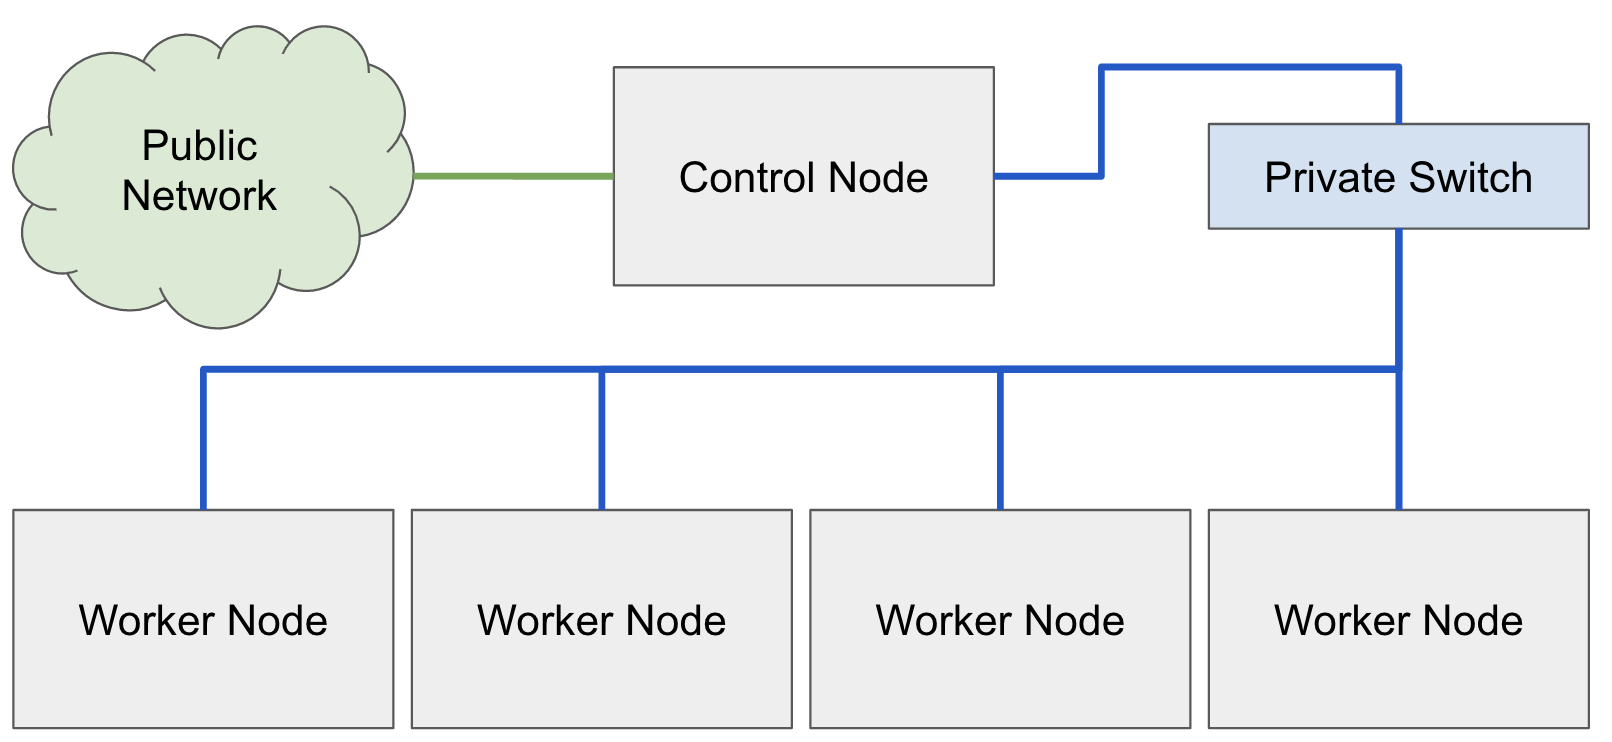
\includegraphics[width=\linewidth]{beowulf_architecture}
\end{block}
\column{0.5\textwidth}
\begin{block}{measurements}
  \begin{itemize}
    \item node image \& system overlay protected with Asset Tag 
    \item system overlays \textbf{must} be downloaded from privileged port
    \item persistant malware installation is impossible as node images are ephermal
  \end{itemize}
\end{block}
\end{columns}
\end{frame}
\begin{frame}[fragile]
\frametitle{Warewulf configuration}
\framesubtitle{Node images}
\begin{columns}
\column{0.5\textwidth}
\begin{block}{ELements}
\begin{itemize}
  \item complete OS images
  \item called containers in warewulf
  \item must be imported from:
  \begin{itemize}
    \item chroot directory
    \item OCI registry
  \end{itemize}
  \item multiple different node images can be imported
  \item node images independent from host OS
\end{itemize}
\end{block}
\column{0.5\textwidth}
\begin{block}{\texttt{registry.suse.com}}
  \begin{itemize}
    \item SUSE SLE 15SP5
  \end{itemize}
\end{block}
\begin{block}{\texttt{registry.opensuse.org}}
  \begin{itemize}
    \item openSUSE Tumleweed
    \item openSUSE Leap 15SP[3-5]
   \end{itemize}
\end{block}
\begin{block}{\texttt{ghcr.io}}
  \begin{itemize}
    \item openSUSE Leap
    \item Rocky EL (8\&9)
    \item Debian Bockworm
  \end{itemize}
\end{block}
\end{columns}
\end{frame}
\begin{frame}[fragile]
\frametitle{Warewulf configuration}
\framesubtitle{Node image examples}
\begin{block}{Import SLE image from SUSE registry}
\begin{lstlisting}[style=wwctl]
ww4-host:# export WAREWULF_OCI_USERNAME=cgoll@suse.com
ww4-host:# export WAREWULF_OCI_PASSWORD=INTERNAL-USE-ONLY-xxxxxx
ww4-host:# wwctl container import docker://registry.suse.com/suse/hpc/warewulf4-x86_64/sle-hpc-node:latest sle-hpc
\end{lstlisting}
\end{block}
\begin{block}{Import Leap image openSUSE registry}
\begin{lstlisting}[style=wwctl]
ww4-host:# wwctl container import docker://registry.opensuse.org/science/warewulf/leap-15.5/containers/kernel:latest leap
\end{lstlisting}
\end{block}
\begin{block}{Execute shell in images}
\begin{lstlisting}[style=wwctl]
wwctl container shell sle-hpc
[sle-hpc] Warewulf>
\end{lstlisting}
\begin{itemize}
  \item SLE registration from outer node is mounted into image
\end{itemize}
\end{block}
\end{frame}
\begin{frame}[fragile]
\frametitle{Warewulf configuration}
\framesubtitle{disk management}
\begin{columns}
\column{0.5\textwidth}
\begin{block}{Needs following elements:}
\begin{itemize}
  \item disks
  \item partitions (on disk)
  \item filesystem (on partition)
\end{itemize}
\end{block}
\begin{block}{Implementation}
  \begin{itemize}
    \item use \texttt{ignition} \\ warewulf has its own service: {ignition-ww4-disk.service}
    \item \textbf{not}  called in \texttt{initrd}
    \item \textbf{before} \texttt{sysroot.mount}
  \end{itemize}
\end{block}
\column{0.5\textwidth}
\begin{block}{Single parition}
\begin{lstlisting}[style=wwctl]
wwctl node set n01 --diskname /dev/vda --diskwipe --partname scratch --partcreate --fsname scratch --fsformat btrfs --fspath /scratch --fswipe
\end{lstlisting}
\end{block}
\begin{block}{Add swap}
\begin{lstlisting}[style=wwctl]
wwctl node set n01 --diskname /dev/vda --partname swap --partsize=1024 --partnumber 1 --fsname swap --fsformat swap --fspath swap
\end{lstlisting}
\end{block}
\end{columns}
\end{frame}
\begin{frame}[fragile]
\frametitle{Warewulf boot}
\framesubtitle{Boot process}
\begin{columns}
\column{0.5\textwidth}
\begin{block}{boot with iPXE}
\begin{itemize}
  \item distribution iPXE binaries are used
  \item \texttt{tftp} transfers are small
  \item \texttt{kernel} is extracted from container/node image on the fly
  \item root fs is the container/node image\\
  configuration overlay added on top
  \item \textbf{no} secure boot
\end{itemize}
\end{block}
\column{0.5\textwidth}
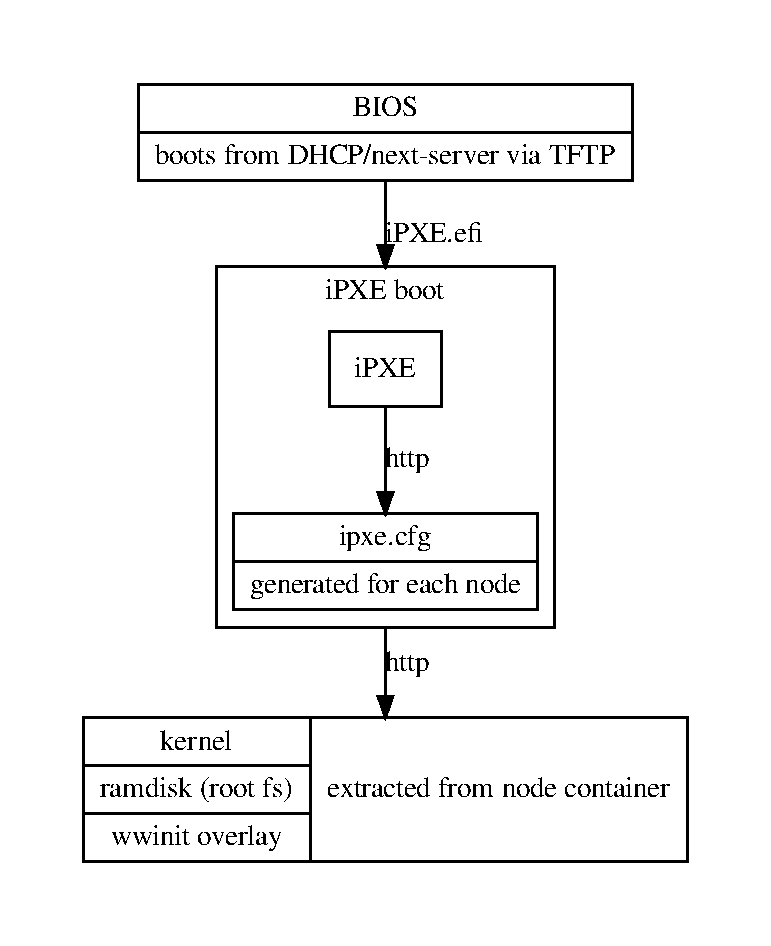
\includegraphics[width=.9\linewidth]{ipxe_boot}
\end{columns}
\end{frame}
\begin{frame}[fragile]
\frametitle{Warewulf boot}
\framesubtitle{Secure boot }
\begin{columns}
\column{0.5\textwidth}
\begin{block}{Boot with grub tftp}
\begin{itemize}
  \item grub \& shim extracted from host
  \item secure boot only possible if host shim \& grub can boot node kernel
\end{itemize}
\end{block}
\column{0.5\textwidth}
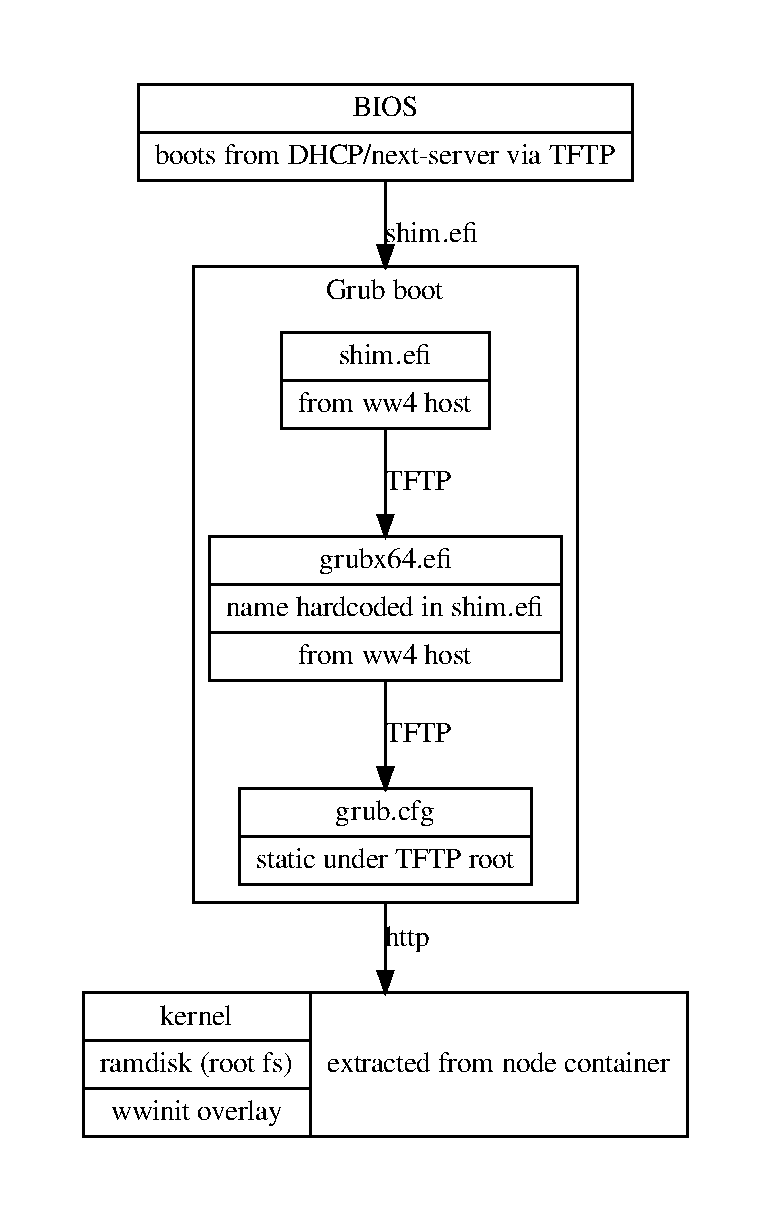
\includegraphics[width=.7\linewidth]{grub_ipxe}
\end{columns}
\end{frame}
\begin{frame}[fragile]
\frametitle{Warewulf secure boot}
\framesubtitle{Cross product secure boot }
\begin{columns}
\column{0.5\textwidth}
\begin{block}{Boot with grub http}
\begin{itemize}
  \item grub \& shim extracted from node/container image
  \item secure boot with various distributions
  \item must be configured in BIOS
\end{itemize}
\end{block}
\column{0.5\textwidth}
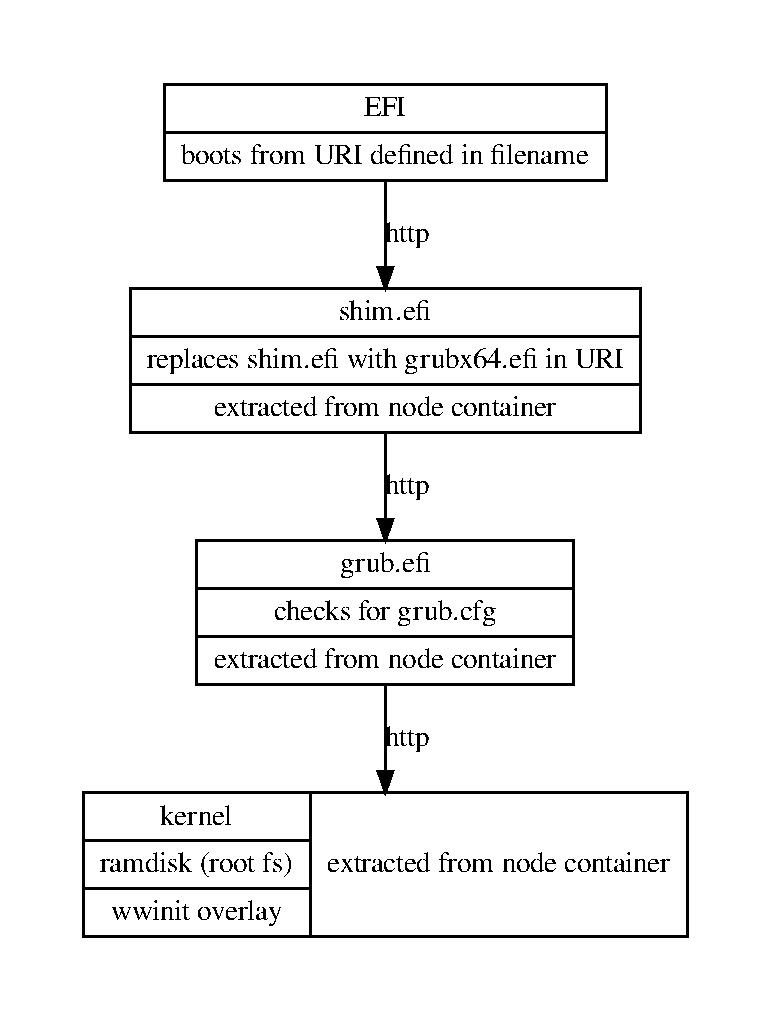
\includegraphics[width=.8\linewidth]{grub_http}
\end{columns}
\end{frame}
\begin{frame}[fragile]
\frametitle{Warewulf}
\framesubtitle{Development}
\begin{columns}
\column{0.5\textwidth}
\begin{block}{Availiability}
  \begin{itemize}
    \item part of SLE since 15SP5
    \item SLE node/container available
  \end{itemize}
\end{block}
\begin{block}{upstream}
\texttt{github.com/warewulf/warewulf} \\
Rocky Linux Foundation project\\
Stakeholders:
\begin{itemize}
  \item SUSE
  \item CIQ
  \item Intel/openHPC
\end{itemize}
\end{block}
\column{0.5\textwidth}

\includegraphics[width=.8\linewidth]{warewulf-logo}
\end{columns}
\end{frame}
\begin{frame}[fragile]
\frametitle{Warewulf}
Thank your, for you attention!
\end{frame}
\end{document}

